\documentclass[]{article}
\usepackage{lmodern}
\usepackage{amssymb,amsmath}
\usepackage{ifxetex,ifluatex}
\usepackage{fixltx2e} % provides \textsubscript
\ifnum 0\ifxetex 1\fi\ifluatex 1\fi=0 % if pdftex
  \usepackage[T1]{fontenc}
  \usepackage[utf8]{inputenc}
\else % if luatex or xelatex
  \ifxetex
    \usepackage{mathspec}
  \else
    \usepackage{fontspec}
  \fi
  \defaultfontfeatures{Ligatures=TeX,Scale=MatchLowercase}
\fi
% use upquote if available, for straight quotes in verbatim environments
\IfFileExists{upquote.sty}{\usepackage{upquote}}{}
% use microtype if available
\IfFileExists{microtype.sty}{%
\usepackage[]{microtype}
\UseMicrotypeSet[protrusion]{basicmath} % disable protrusion for tt fonts
}{}
\PassOptionsToPackage{hyphens}{url} % url is loaded by hyperref
\usepackage[unicode=true]{hyperref}
\PassOptionsToPackage{usenames,dvipsnames}{color} % color is loaded by hyperref
\hypersetup{
            pdftitle={Messy Notes for Applied},
            pdfauthor={Kexing Ying},
            colorlinks=true,
            linkcolor=Maroon,
            citecolor=Blue,
            urlcolor=red,
            breaklinks=true}
\urlstyle{same}  % don't use monospace font for urls
\usepackage[margin = 1.5in]{geometry}
\usepackage{graphicx,grffile}
\makeatletter
\def\maxwidth{\ifdim\Gin@nat@width>\linewidth\linewidth\else\Gin@nat@width\fi}
\def\maxheight{\ifdim\Gin@nat@height>\textheight\textheight\else\Gin@nat@height\fi}
\makeatother
% Scale images if necessary, so that they will not overflow the page
% margins by default, and it is still possible to overwrite the defaults
% using explicit options in \includegraphics[width, height, ...]{}
\setkeys{Gin}{width=\maxwidth,height=\maxheight,keepaspectratio}
\IfFileExists{parskip.sty}{%
\usepackage{parskip}
}{% else
\setlength{\parindent}{0pt}
\setlength{\parskip}{6pt plus 2pt minus 1pt}
}
\setlength{\emergencystretch}{3em}  % prevent overfull lines
\providecommand{\tightlist}{%
  \setlength{\itemsep}{0pt}\setlength{\parskip}{0pt}}
\setcounter{secnumdepth}{5}
% Redefines (sub)paragraphs to behave more like sections
\ifx\paragraph\undefined\else
\let\oldparagraph\paragraph
\renewcommand{\paragraph}[1]{\oldparagraph{#1}\mbox{}}
\fi
\ifx\subparagraph\undefined\else
\let\oldsubparagraph\subparagraph
\renewcommand{\subparagraph}[1]{\oldsubparagraph{#1}\mbox{}}
\fi

% set default figure placement to htbp
\makeatletter
\def\fps@figure{htbp}
\makeatother

\usepackage{tikz}
\usepackage{amsthm}
\usepackage{mathtools}
\usepackage[ruled,vlined]{algorithm2e}
\newtheorem{theorem}{Theorem}
\newtheorem{corollary}{Corollary}[theorem]
\newtheorem*{remark}{Remark}

\title{Messy Notes for Applied}
\author{Kexing Ying}
\date{May 15, 2020}

\begin{document}
\maketitle

{
\hypersetup{linkcolor=black}
\setcounter{tocdepth}{2}
\tableofcontents
}
\newpage

\section{Circuits}\label{circuits}

In this section we will discuss the method of using matrices in solving
the potiential and conductance problem regarding circuits.

I will assume you can manipulate matrices and use basic linear algebra,
I will also assume you can construct the incidence matrix of a graph.

\subsection{Null-Spaces}\label{null-spaces}

Consider an incidence matrix \(A\) representing a circuit.

Then (if we let \(\Phi\) be the vector representing the potiential at
each node) we have \(A \Phi = w\)~is the potiential difference across
each edge.

With this, we see that there is the trivial right null-vector
\(\Phi_0 = \left(\mathbf{1} \right)\), as if each node has the same
potiential, the the potiential difference across each edge is zero. In
fact, this is the \textbf{only} linearly independent right null-vector
of \(A\) (given that the circuit is connected) since if there is two
nodes that have different potiential, then of course there is going to
be some edge with some potiential difference.

On the other hand, for \(-A^T w = f\) where \(w\) is the potiential
difference across each node, we have \(f\)~being the vector representing
the \emph{sum} of the potientials out of each node.

Then the dimension of the left null-space of \(A\) is represented by the
number of ``loops'' of the circuit and we can find the basis of the left
null-space by the following method:

\begin{enumerate}
\def\labelenumi{\arabic{enumi}.}
\item
  Let \(w_i \in \mathbb{R}^n\)~be the vector representing the path of a
  loop where \(n\) is the number of edges of the circuit.
\item
  For each edge the path traverses, put a \(1\) in that position if the
  path follows the directed graph and a \(-1\) if it goes against it.
\item
  Fill in the rest with \(0\)s.
\end{enumerate}

Thus, by rank-nullity, we can easily verify our previous statement that
the trivial right-null vector is the only right-null vector.

\subsection{Connected Graphs}\label{connected-graphs}

The question is what happens when we have two disconnected graphs
representing a single graph?

Well, with two disconnected graphs, we can see there are two trivial
right-null vectors, i.e.
\(\Phi_0 = \left(\mathbf{1}, \mathbf{0} \right)\) and
\(\Phi_0' = \left(\mathbf{0}, \mathbf{1} \right)\). We can easily see
that our original trivial null-vector is in the span of these two new
null-vectors.

\subsection{Useful Terms}\label{useful-terms}

\begin{itemize}
\item
  \(A\) is the \emph{incidence matrix} of the graph
\item
  \(K = A^T A\) is the \emph{Laplacian matrix} of the graph
\item
  \(C = \text{diag}(c_1, \dots c_n)\) the \emph{conductance} matrix of
  the graph
\item
  \(K_c = A^T C A\) is the \emph{weighted Laplacian matrix} of the graph
\item
  \(-A^Tw\) is called the \emph{divergence} of the currents (at the
  nodes)
\item
  \(C_{e}\) is the \emph{effective conductance} of a circuit
\end{itemize}

\subsection{KCL Cannot Hold at All
nodes!}\label{kcl-cannot-hold-at-all-nodes}

Consider the result from the \emph{fundamental theorem of linear
algebra}:

\begin{itemize}
\tightlist
\item
  The null space of \(A^T\) is orthogonal to the row space of \(A\),
  i.e. \(\ker A^T \perp \text{csp} A\).
\end{itemize}

(This is true because if \(v \in \ker A\), then the dot product of \(v\)
and the rows of \(A\) must be zero, so it must be perpendicular to the
row vectors of \(A\). But for all \(w \in \text{rsp} A\), \(w\) is a
linear combination of the row vectors of \(A\), so \(v \cdot w = 0\) and
hence, as \(\text{rsp} A = \text{csp} A^T\), we have
\(\ker A \perp \text{csp} A^T\).)

With that, let use suppose \emph{KCL} holds at all the nodes. Then, we
have \(\mathbf{0} = A^T w\) for some \(w\) representing the potiential
difference across each edge. Then, by definition, \(w\) is in the
null-space of \(A^T\). But this, by our aforementioned lemma must be
perpendicular to any vectors in \(\text{csp} A = \text{Im} A\) and
hence, if \(w \neq 0\) (which we are assuming as otherwise we would have
a circuit not doing anything!) there does not exist some potiential
vector \(\Phi\) such that \(w = A\Phi\).

Physically, this means that under the assumption that \emph{KCL} holds
at all nodes, there will be \textbf{no} non-trivial potiential that will
produce a current through our circuit (but of course the trivial
null-vectors of \(A\) satisfy our equation \(\mathbf{0} = A^T A \Phi\)).

\subsection{Method for Finding the
Potientials}\label{method-for-finding-the-potientials}

Just solve \[ f = A^T C A \Phi = K_c \Phi \] and we are done!

Okay, perhaps this is not very helpful so to expand on what I've said
above, let us consider two types of questions.

\subsubsection{Specified Conductance}\label{specified-conductance}

First, perhaps we are given the net currents at the boundary nodes, i.e.
\(f\)~is known and we are asked to find \(\Phi\) such that
\(f = K_c \Phi\). Then, you might just think to do something like
\(\Phi = K_c ^{-1} f\) to determine \(\Phi\). But this is no good as
\(K_c\) is singular and therefore not invertible (recall that we have
the trivial null-vector for \(A\), \(\Phi_0\) so
\(K_c \Phi_0 = A^T C (A\Phi_0) = A^T C \mathbf{0} = \mathbf{0}\)). So
what we do is we set one of the nodes to have potiential zero, i.e.~we
will have that node as our reference potiential (if you think about this
physically what I'm saying is that the potiential at one node doesn't
really mean much - its the potiential difference that actually does the
work so fixing one node potiential doens't effect what we are really
after - the potiential difference).

So what we do have now is some mathematical trickery. If we fix the
\(i\)-th nodes to have potiential zero, then when we multiply \(K_c\)
with this potiential vector, you can see that the \(i\)-th row and
collumn of \(K_c\) nolonger contribute to the multiplication so by
removing them, we receive a new linear system \(K_c' \Phi' = f'\). Now,
by repeating this process until its solvable, we should receive some
vector \(\bar{x}\) that is satisfied by our original system and hence we
have a solution space
\[S = \bar{x} + \ker A := \{\bar{x} + x_0 \mid x_0 \in \ker A \}.\]

\subsubsection{Specified Potientials}\label{specified-potientials}

So now what if we are given the potientials at the boundary nodes and
are asked to find the potientials at the non-boundary nodes while also
finding the net-currents out of the boundary nodes?

Well, thats a lot asked from us, but I think we can manage. So in this
case we have \(K_c \Phi = f\) where \(\Phi = (x_1, x_2, x_3, \dots)^T\)
and \(f = (f_1, -f_1, 0, \dots)^T\) where \(x_1, x_2\) are given and we
are asked to find the rest (if it's not in this form then just rewrite
it in this form). And then all we have to do is to use the
\href{https://en.wikipedia.org/wiki/Schur_complement}{Schur complement}
and Wikipedia can explain the rest.

One more comment. The effective conductance of the system \(C_e = f_1\).

\subsection{Calculating the Effective
Conductance}\label{calculating-the-effective-conductance}

We will now present some trickery in calculating the effective
conductance of a circuit by simplifying the circuit whenever we see
edges in series or parallel.

\subsubsection{Edges in Parallel}\label{edges-in-parallel}

Suppose we have the following graph represting a particular section of
another graph with parallel edges.

\begin{center}

\tikzset{every picture/.style={line width=0.75pt}} %set default line width to 0.75pt        

\begin{tikzpicture}[x=0.75pt,y=0.75pt,yscale=-1,xscale=1]

%Shape: Ellipse [id:dp829851062863453] 
\draw   (160.7,220.4) .. controls (160.7,209.35) and (198.67,200.4) .. (245.5,200.4) .. controls (292.33,200.4) and (330.3,209.35) .. (330.3,220.4) .. controls (330.3,231.45) and (292.33,240.4) .. (245.5,240.4) .. controls (198.67,240.4) and (160.7,231.45) .. (160.7,220.4) -- cycle ;
%Shape: Circle [id:dp9737682550697424] 
\draw  [fill={rgb, 255:red, 0; green, 0; blue, 0 }  ,fill opacity=1 ] (157.95,220.4) .. controls (157.95,218.88) and (159.18,217.65) .. (160.7,217.65) .. controls (162.22,217.65) and (163.45,218.88) .. (163.45,220.4) .. controls (163.45,221.92) and (162.22,223.15) .. (160.7,223.15) .. controls (159.18,223.15) and (157.95,221.92) .. (157.95,220.4) -- cycle ;
%Shape: Circle [id:dp35076255197956563] 
\draw  [fill={rgb, 255:red, 0; green, 0; blue, 0 }  ,fill opacity=1 ] (327.55,220.4) .. controls (327.55,218.88) and (328.78,217.65) .. (330.3,217.65) .. controls (331.82,217.65) and (333.05,218.88) .. (333.05,220.4) .. controls (333.05,221.92) and (331.82,223.15) .. (330.3,223.15) .. controls (328.78,223.15) and (327.55,221.92) .. (327.55,220.4) -- cycle ;

% Text Node
\draw (234,185) node [anchor=north west][inner sep=0.75pt]    {$c_{a}$};
% Text Node
\draw (236,245) node [anchor=north west][inner sep=0.75pt]    {$c_{b}$};
% Text Node
\draw (146,210.4) node [anchor=north west][inner sep=0.75pt]    {$1$};
% Text Node
\draw (334,210.4) node [anchor=north west][inner sep=0.75pt]    {$2$};

\end{tikzpicture}

\end{center}

Let us write out the incidence matrix and the conductance matrix, \[
A =
\begin{pmatrix}
-1 & 1 \\ -1 & 1
\end{pmatrix},
\hspace{2mm}
C = 
\begin{pmatrix}
c_a & 0 \\ 0 & c_b
\end{pmatrix}.
\] Then, if let the system have unit potiential at node 1 and zero
potiential at node 2, we have \[
f = A^T C A \Phi = 
\begin{pmatrix}
-1 & -1 \\ 1 & 1
\end{pmatrix}
\begin{pmatrix}
c_a & 0 \\ 0 & c_b
\end{pmatrix}
\begin{pmatrix}
-1 & 1 \\ -1 & 1
\end{pmatrix}
\begin{pmatrix}
1 \\ 0
\end{pmatrix}
=
\begin{pmatrix}
c_a + c_b \\ -(c_a + c_b)
\end{pmatrix}
\] implying that for edges in parallel, we shall add the conductance.

\subsubsection{Edges in Series}\label{edges-in-series}

It's a very similar story for edges in series but the matrices doesn't
multiply as nicely so we will omit it the proof but the result is that
given the below graph,

\begin{center}

\tikzset{every picture/.style={line width=0.75pt}} %set default line width to 0.75pt        

\begin{tikzpicture}[x=0.75pt,y=0.75pt,yscale=-1,xscale=1]
%uncomment if require: \path (0,300); %set diagram left start at 0, and has height of 300

%Shape: Circle [id:dp35076255197956563] 
\draw  [fill={rgb, 255:red, 0; green, 0; blue, 0 }  ,fill opacity=1 ] (327.55,219.4) .. controls (327.55,218.88) and (328.78,217.65) .. (330.3,217.65) .. controls (331.82,217.65) and (333.05,218.88) .. (333.05,220.4) .. controls (333.05,221.92) and (331.82,223.15) .. (330.3,223.15) .. controls (328.78,223.15) and (327.55,221.92) .. (327.55,220.4) -- cycle ;
%Shape: Circle [id:dp9417251220811065] 
\draw  [fill={rgb, 255:red, 0; green, 0; blue, 0 }  ,fill opacity=1 ] (242.95,219.4) .. controls (242.95,218.88) and (244.18,217.65) .. (245.7,217.65) .. controls (247.22,217.65) and (248.45,218.88) .. (248.45,220.4) .. controls (248.45,221.92) and (247.22,223.15) .. (245.7,223.15) .. controls (244.18,223.15) and (242.95,221.92) .. (242.95,220.4) -- cycle ;
%Shape: Circle [id:dp0686829237101314] 
\draw  [fill={rgb, 255:red, 0; green, 0; blue, 0 }  ,fill opacity=1 ] (156.95,219.4) .. controls (156.95,217.88) and (158.18,216.65) .. (159.7,216.65) .. controls (161.22,216.65) and (162.45,217.88) .. (162.45,219.4) .. controls (162.45,220.92) and (161.22,222.15) .. (159.7,222.15) .. controls (158.18,222.15) and (156.95,220.92) .. (156.95,219.4) -- cycle ;
%Straight Lines [id:da5944259677353316] 
\draw    (159.7,219.4) -- (330.3,219.4) ;

% Text Node
\draw (191,205.4) node [anchor=north west][inner sep=0.75pt]    {$c_{a}$};
% Text Node
\draw (283,205.4) node [anchor=north west][inner sep=0.75pt]    {$c_{b}$};
% Text Node
\draw (146,210.4) node [anchor=north west][inner sep=0.75pt]    {$1$};
% Text Node
\draw (334,210.4) node [anchor=north west][inner sep=0.75pt]    {$2$};

\end{tikzpicture}

\end{center}

we can treat the system as one edge with conductance
\(c_ac_b/(c_a + c_b)\).

\section{Random Walks}\label{random-walks}

In this section, we shall examine another system - random walks on a
graph and explore its similarity to a circuit system. With this, we will
conclude that in fact the two systems are the same and are said to be
\emph{harmonic} and for each method of solving the specific problem, an
equivalent method can be used for the other.

We shall also consider two additional methods for solving problems
involving harmonic graphs - \emph{algebraic} and the \emph{method of
relaxation}.

\subsection{A Stroll Through Central
London}\label{a-stroll-through-central-london}

Consider the much reduced (an worse) tubemap of central London,

\begin{figure}
\centering
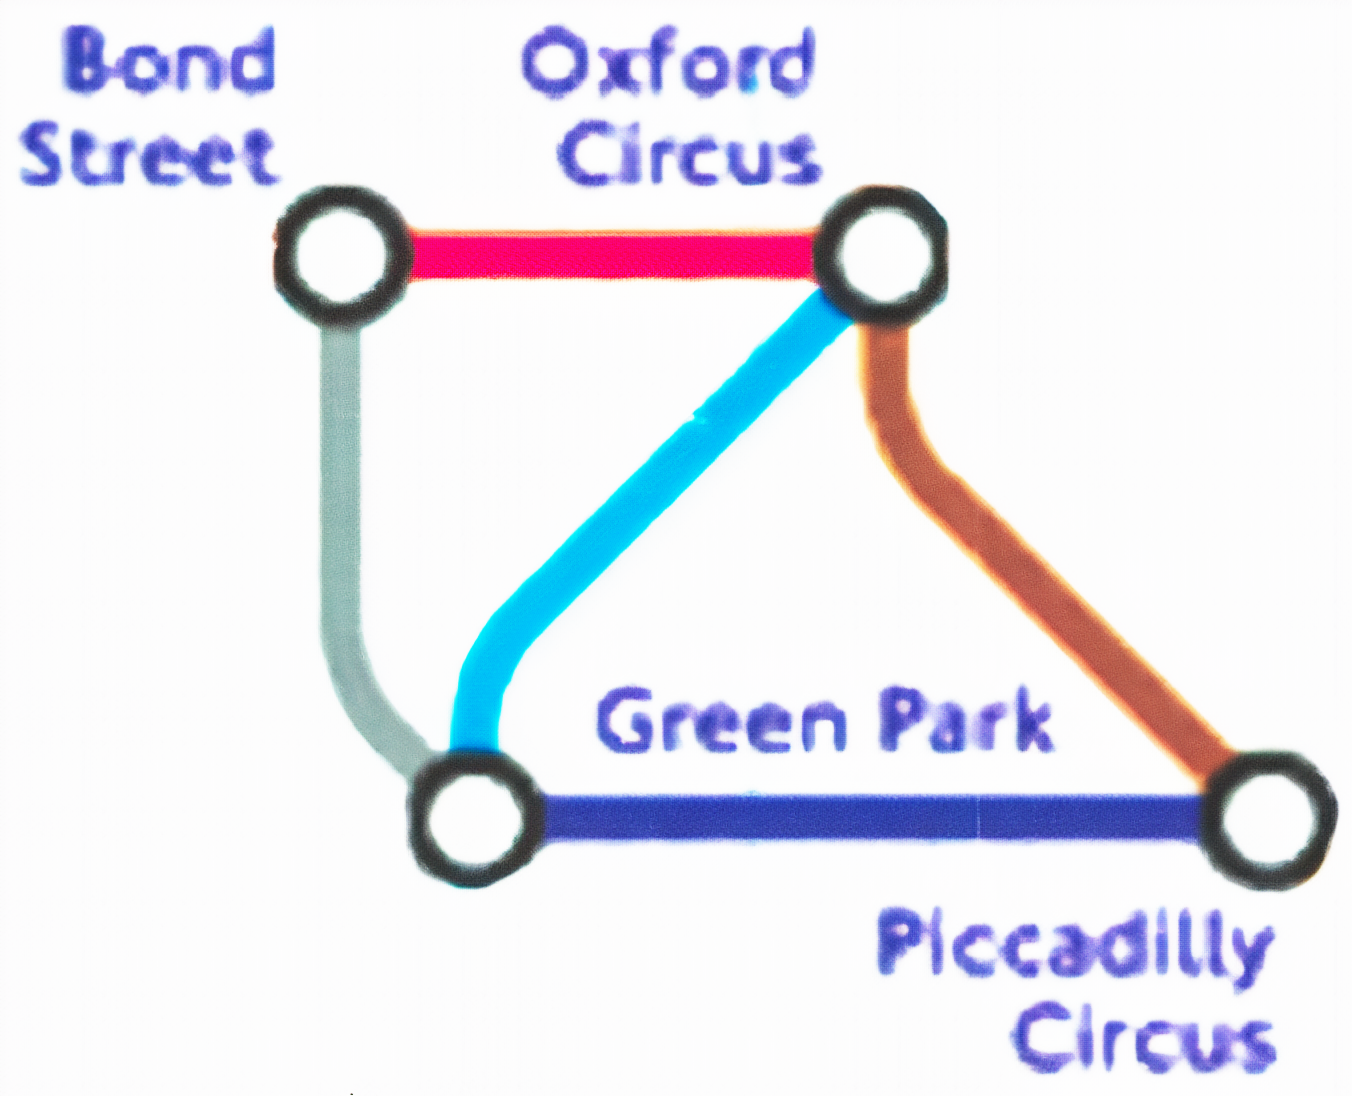
\includegraphics[height=1.5in]{./walk.png}
\caption{A fictional tubemap of central London.}
\end{figure}

and suppose, your very drunk friend, Xin, gotten himself wasted at
\emph{Station \(A\)}. Wanting to get home, Xin takes a random tube at
each station and gets off at the next rinse and repeat until he reaches
some station we will specify.

We would now like to pose three questions:

\begin{enumerate}
\def\labelenumi{\arabic{enumi}.}
\item
  What is the probability that, if Xin starts at \emph{Oxford Circus},
  he reaches \emph{Bond Street} before reaching \emph{Green Park}?
\item
  What is the probability if Xin starts at \emph{Piccadilly Circus}
  instead?
\item
  What is the probability that if Xin starts as \emph{Bond Steet} and
  leaves, he reaches \emph{Green Park} rather than returning to
  \emph{Bond Street}?
\end{enumerate}

\subsubsection{An Recursive Algorithm for Question
1}\label{an-recursive-algorithm-for-question-1}

Often times, it is helpful to first simulate our problem with a computer
programme so we can see perhaps there is a pattern to our answer. To
achieve this however, there are many different methods. Here I have
prepared a pseudocode representation for a recursive implementation of
simulating one random walk however there are different ways of achieving
the same without recursions.

\begin{algorithm}[H]
  \SetAlgoLined
  \SetKwFunction{FMain}{walkNext}
  \SetKwProg{Fn}{Function}{:}{}

  \SetKwFunction{CStation}{stations}
  \SetKwProg{Cl}{Class}{:}{}

  \SetKw{kwLet}{let}
  \SetKw{kwChoose}{choose from}
  
  \Cl{\CStation{name, connected}}{
    \kwLet{self.name = name}\;
    \kwLet{self.connected = connected}\;
  }

  \Fn{\FMain{currentStation}}{
    \eIf{currentStation $\neq$ bondStreet $\lor$ greenPark}{
      \FMain{\kwChoose{currentStation.connected}}\;    
    }{
      \Return{currentStation}
    }
  }
 \caption{An recursive method of simulating random walks}
\end{algorithm}

By making each station a data structure containing its name and its
adjacent stations, we can recursively choose the next station until we
reach Bond Street or Green Park.

\begin{algorithm}[H]
  \SetAlgoLined
  \SetKwFunction{FMain}{walkNext}
  \SetKw{kwPass}{Pass}
  \SetKw{kwLet}{let}

  \kwLet{reachedBondStreet = 0}\;

  \While{runs $\le$ $n$} {
    \eIf{\FMain{oxfordCircus} $=$ bondStreet}{
      bondStreet += 1\;
    }{
      \kwPass
    }
    runs += 1\;
  }

  \kwLet{probability = $reachedBondStreet/n$}
 \caption{Finding the probability given our method of simulating one random walk}
\end{algorithm}

Thus, by doing sufficiently large number of such random walks, we can
compare the ratio of the number times Xin reached Bond Street against
the total number of runs.

By implementing this algorithm in an actual programming language, it
seems that this probability appears to be around \(2 / 5\) which is
exactly the same value if we attempted to compute this as if this was a
circuit with unit conductances on each edge.

This is surprising as on the surface, neither systems seemed to have
anything to do with each other, but however, later we will find out that
both systems are \emph{harmonic} and therefore are essentially the same.

\subsection{An Algebraic Method}\label{an-algebraic-method}

As promised, I will now present an algebraic method in solving the
random walker problem.

Let use first rephrase the question so we can refer to it easier.
Consider the graph drawn below. We can easily see that the graph and the
tubemap are infact the same with Bond Street being node 1, Green Park as
node 2 and so on.

With that, we can rephrase the question such that we are asked to find
\(p_3\) where \(p_i\) represents the probability of reaching node 1
before reaching node 4.

Consider the \emph{law of total probability}:

\begin{itemize}
\tightlist
\item
  Given a event \(E \in \mathcal{F}\) and
  \(B = \{B_i | i \in \mathcal{I}\} \subseteq \mathcal{F}\)~ for some
  index set \(\mathcal{I}\), if \(B\) forms a partition of the sample
  space \(\Omega\), then \[
  P(E) = \sum_{i \in \mathcal{I}}P(E | B_i)P(B_i).
  \]
\end{itemize}

\begin{figure}
\centering
\tikzset{every picture/.style={line width=0.75pt}} %set default line width to 0.75pt        

\begin{tikzpicture}[x=0.75pt,y=0.75pt,yscale=-1,xscale=1]
%uncomment if require: \path (0,300); %set diagram left start at 0, and has height of 300

%Shape: Circle [id:dp35076255197956563] 
\draw  [fill={rgb, 255:red, 0; green, 0; blue, 0 }  ,fill opacity=1 ] (323.55,162.4) .. controls (323.55,160.88) and (324.78,159.65) .. (326.3,159.65) .. controls (327.82,159.65) and (329.05,160.88) .. (329.05,162.4) .. controls (329.05,163.92) and (327.82,165.15) .. (326.3,165.15) .. controls (324.78,165.15) and (323.55,163.92) .. (323.55,162.4) -- cycle ;
%Shape: Circle [id:dp9417251220811065] 
\draw  [fill={rgb, 255:red, 0; green, 0; blue, 0 }  ,fill opacity=1 ] (233.95,102.4) .. controls (233.95,100.88) and (235.18,99.65) .. (236.7,99.65) .. controls (238.22,99.65) and (239.45,100.88) .. (239.45,102.4) .. controls (239.45,103.92) and (238.22,105.15) .. (236.7,105.15) .. controls (235.18,105.15) and (233.95,103.92) .. (233.95,102.4) -- cycle ;
%Shape: Circle [id:dp0686829237101314] 
\draw  [fill={rgb, 255:red, 0; green, 0; blue, 0 }  ,fill opacity=1 ] (142.95,161.4) .. controls (142.95,159.88) and (144.18,158.65) .. (145.7,158.65) .. controls (147.22,158.65) and (148.45,159.88) .. (148.45,161.4) .. controls (148.45,162.92) and (147.22,164.15) .. (145.7,164.15) .. controls (144.18,164.15) and (142.95,162.92) .. (142.95,161.4) -- cycle ;
%Straight Lines [id:da5944259677353316] 
\draw    (145.7,161.4) -- (236.7,102.4) ;
%Straight Lines [id:da6450577900800967] 
\draw    (236.7,102.4) -- (326.3,162.4) ;
%Shape: Circle [id:dp24894190681032202] 
\draw  [fill={rgb, 255:red, 0; green, 0; blue, 0 }  ,fill opacity=1 ] (233.55,222.4) .. controls (233.55,220.88) and (234.78,219.65) .. (236.3,219.65) .. controls (237.82,219.65) and (239.05,220.88) .. (239.05,222.4) .. controls (239.05,223.92) and (237.82,225.15) .. (236.3,225.15) .. controls (234.78,225.15) and (233.55,223.92) .. (233.55,222.4) -- cycle ;
%Straight Lines [id:da3966263499064042] 
\draw    (145.7,161.4) -- (236.3,222.4) ;
%Straight Lines [id:da1821539361067317] 
\draw    (236.7,102.4) -- (236.3,222.4) ;
%Straight Lines [id:da3374921124672794] 
\draw    (326.3,162.4) -- (236.3,222.4) ;

% Text Node
\draw (132,152.4) node [anchor=north west][inner sep=0.75pt]    {$1$};
% Text Node
\draw (330,153.6) node [anchor=north west][inner sep=0.75pt]    {$2$};
% Text Node
\draw (231,80.6) node [anchor=north west][inner sep=0.75pt]    {$3$};
% Text Node
\draw (230,227.6) node [anchor=north west][inner sep=0.75pt]    {$4$};
% Text Node
\draw (173,187.6) node [anchor=north west][inner sep=0.75pt]    {$a$};
% Text Node
\draw (289,188.6) node [anchor=north west][inner sep=0.75pt]    {$b$};
% Text Node
\draw (173,120.6) node [anchor=north west][inner sep=0.75pt]    {$c$};
% Text Node
\draw (290,119.6) node [anchor=north west][inner sep=0.75pt]    {$d$};
% Text Node
\draw (223,153.6) node [anchor=north west][inner sep=0.75pt]    {$e$};

\end{tikzpicture}
\caption{A graph representation of the tubemap.}
\end{figure}

Then, starting at node 3, we see that Xin can either go to node 1, 2 or
4, so the events of Xin going to node 1, node 2 and goint to node 4
partitions the sample space. Therefore by the law of total probability,
we have \[
p_3 = \frac{1}{3} \times p_1 + \frac{1}{3} \times p_2 + \frac{1}{3} \times p_4.
\] Similarily, we see that going to node 3 or node 4 from node 2
partitions the sample space, so \[
p_2 = \frac{1}{2} \times p_3 + \frac{1}{2} \times p_4.
\] Now, if we started from node 4, then there is of course no change of
reaching node 1 before node 4 (as you are aleady at node 4!) so
\(p_4 = 0\). Similarily if we started from node 1, then the probability
of reaching 1 before 4 is 1, so \(p_1 = 1\).

Thus, by plugging in \(p_1 = 1\) and \(p_4 = 0\), we have a system of
equations with two unknowns, \[
\begin{split}
p_3 & = \frac{1}{3} + \frac{1}{3} \times p_2 \\
p_2 & = \frac{1}{2} \times p_3
\end{split}
\] which is easily solvable resulting in \(p_3 = 2 / 5\) and
\(p_2 = 1 / 5\) would you imagine it! It's exactly what we expected from
the simulated solution (and the same solution as the matrix method).

\subsection{Connection Between the Two
Systems}\label{connection-between-the-two-systems}

Recall our equation for circuits, \(f = K \Phi\) where in which at the
non-boundary nodes, we had the enforcement of \emph{KCL}. So suppose
\(\phi_i\) is the potiential at a non-boundary node. As \emph{KCL} is
upheld at this node, we have the \(i\)-th row of \(K \Phi\) being zero.
So by denoting \(\deg(i)\) by the number of edges connected to node
\(i\), we have \[
\deg(i) x_i - \sum_{\mathclap{\substack{j \in \text{connected}\\ \text{nodes}}}} x_j = 0,
\] so by rearranging, we have,

\begin{equation}
x_i = \sum_{\mathclap{\substack{j \in \text{connected}\\ \text{nodes}}}} x_j/ \deg(i),
\end{equation}

which is exactly what we have done for the algebraic method for random
walks.

\subsubsection{Intuitive Interpretation}\label{intuitive-interpretation}

Intuitively we can interpret both system as graphs with some variables
associated with the nodes. Furthermore, as demonstrated by the above
equation, we see that in both system, the node variable of each node is
the \textbf{average} of the its neighbouring node variables. In the case
of circuits, the potientials (the node variable) of each node is the
average of its neighbours (assuming uniform conductance) and similarly
in the case of the random walk, the probability (the node variable) is
the average of its neighbours (assuming each path is equally likely).

With that, we can abstract graph systems such as these in which each
nodes of the graph is associated with a node variable that is the
average of its neighbouring nodes and we will call such systems
\emph{harmonic}.

And thus, as these systems are essentially the same in our framework, we
can utilize a method of one system interchangably with another.

\subsubsection{Weighted Harmonic Graphs}\label{weighted-harmonic-graphs}

However, what if our conductances/ probabilites of going to each
neighbouring stations are not the same? Then we shall call the harmonic
system \emph{weighted}.

As an extention of the regular harmonic system, we see that we do not
need to change our original framework much but to weight each node
variable according to the conductances/ probabilites or whatever other
system we are using resulting in

\begin{equation}
x_i = \sum_{\mathclap{\substack{j \in \text{connected}\\ \text{nodes}}}} (x_j/ c_j),
\end{equation}

where \(c_j\) denotes the weight we have assigned to the edge connecting
the \(i\)-th node and the \(j\)-th node.

\subsection{Method of Relaxation}\label{method-of-relaxation}

With our interpretation in mind, we can now construct another algorithm
that converges to our desired node variables by averaging the each node
variables with the adjacent ones (with weighing dependent one the edge
variables if the edge variables are not uniform) over and over agains
for sufficiently large number of times.

Below are some pseudocode describing this method.

We first create a object called \(\tt{Node}\) containing information
about its neighbours and it's initial potiential and we will let a
\(\tt{graph}\) to be a collection of \(\tt{node : Node}\).

\begin{algorithm}[H]
  \SetAlgoLined
  \SetKwFunction{CNodes}{Node}
  \SetKwProg{Cl}{Class}{:}{}

  \SetKw{kwLet}{let}
  \SetKw{kwDec}{declared}
  
  \Cl{\CNodes{name, nodeVariable, connected, weighing}}{
    \kwLet{self.name = name}\;
    \kwLet{self.connected = connected}\;
    \kwLet{self.$weighing_i$ = $weighing_i$}\;
    \eIf {\kwDec{nodeVariable}}{
      \kwLet{self.nodeVariable = nodeVariable}\;
      \kwLet{self.boundary = True}

    }{
      \kwLet{self.nodeVariable = 0}\;
      \kwLet{self.boundary = False}
    }
  }
  \kwLet{graph = $\{node_1, node_2, \cdots, node_k\}$}\;
 \caption{Constructing the object of nodes and creating a graph as a set of nodes}
\end{algorithm}

Then by looping over all the non-boundary nodes for sufficient amount of
times the node variables of each node converges to the true value.

\begin{algorithm}[H]
  \SetAlgoLined
  \SetKw{kwLet}{let}
  \SetKw{kwPass}{Pass}
  
  \While{runs $\le$ $n$}{
    \For {node $\in$ graph $\land$ node.boundary $=$ False} {
      node.nodeVariable = $\sum\limits_{\mathclap{i \in node.connected}} weighing_i \times node_i.nodeVariable$
    }
    runs += 1
  } 
 \caption{Constructing the object of nodes and creating a graph as a set of nodes}
\end{algorithm}

\section{Harmonic Graphs}\label{harmonic-graphs}

In this section we shall examine some properties of harmonic graphs.

\subsection{Maximum Principle}\label{maximum-principle}

Given a harmonic graph, it is rather natural to seperate its nodes into
\emph{boundary nodes} and \emph{internal nodes} (all other nodes). Then
the \emph{maximum principle} states the following:

\begin{itemize}
\tightlist
\item
  For a harmonic graph, the node variables attains maximum and minimum
  at the boundary nodes.
\end{itemize}

To see why this is true recall that for a (weighted) harmonic graph,
each internal node has node variable that is a weighted average of its
neighbouring node variables. So if a harmonic graph attains its maximum
node variable at a internal node, then all nodes adjacent must be less
equal to it. However, as the node variable is the weighted average of
the adjacent node variables, if there is one adjacent node variable
strictly less than it, the weighted average will be smaller resulting in
a contradiction. Therefore, all adjacent nodes must have the same node
variable as the maximum. Now repeat this until it reaches a boundary
node, resulting in our original statement.

The same argument works for the minimum.

\subsection{Uniqueness Principle}\label{uniqueness-principle}

Given two harmonic graphs, the uniqueness principle states that if the
graphs have the same boundary conditions (and the same edge variables if
it is not uniform), then they also have the same node variables
everywhere.

This is true because if we let \(x_i\) and \(p_i\) denote the \(i\)-th
node variable of the two graphs, then the graph with node variables
defined by \(d_i = x_i - p_i\)~attains maximum and minimum at one of its
boundary nodes. But at the boundary nodes, \(x_i = p_i\) implying
\(\max_j d_j = \min_j dj = 0\) and hence has node variable zero
everywhere.

This is a very important principle as this ensures that our solution for
the random walk problem is the same as the circuit and is the same for
any other harmonic graphs for that matter!

\subsection{Dirichlet's Principle}\label{dirichlets-principle}

The energy dissipation associated with any circuit with two boundary
nodes with potiential 1 and 0 is defined to be \[
\xi(\Phi) = \Phi^T K \Phi
\] where \(K\) is the (weighted) Laplacian and \(\Phi\) is any
potiential vector.

Dirichlet's principle states that the potential vector \(\Phi_*\)
satisfying \emph{KCL} at all internal nodes minimizes the energy
dissipation, i.e. \[\xi(\Phi_*) = \min_\Phi \xi(\Phi).\]

\subsection{Thomson's Principle}\label{thomsons-principle}

By mathematical manipulation the energy dissipation from a circuit can
also be written as \[
\begin{split}
\xi(\Phi) = \Phi^T K \Phi & = \Phi^T A^T C A \Phi\\
& = (-A \Phi)^T (-CA \Phi)\\
& = \sum_{\mathclap{k \in \text{edges}}} w_k\left(\frac{w_k}{c_k}\right)\\
& = \hat{\xi}(w),
\end{split}
\] where \(w_k\) is the current in the \(k\)-th edge and \(c_k\) is the
conductance in the \(k\)-th edge.

Notice that this new expression of energy dissipation does not have
potiential as it's variable but the edge currents. So as a corollary of
Dirichlet's principle, the current vector such that all the internal
nodes satisfies \emph{KCL} also minimizes energy dissipation.

\subsection{Tellegen's Theorem}\label{tellegens-theorem}

Given a circuit with incidence matrix \(A\) and any vector \(w\)
satisfying \emph{KCL} at all nodes (\(w\) does not need to equal some
\(A\Phi\) for some potiential vector \(\Phi\)), then for any \(e\) a
potiential difference vector, Tellegen's theorem states,
\[ e^T w = \mathbf{0}. \]

\begin{proof}
Since $e$ is some vector of potiential difference, then there exist some $\Phi \in \mathbb{R}^n$, a potiential 
vector, such that $e = -A\Phi$. Thus
\begin{align*}
e^T w = (- A\Phi)^T w & = - \Phi^T A^T w \\
& = - \Phi^T (w^T A)^T\\
& = - \Phi^T \mathbf{0} = \mathbf{0}
\end{align*}
as required.
\end{proof}

Now suppose that \(w\) is some vector that satisfies \(-A^T w = f\) then
for all \(e\) a potiential difference vector such that \(e = -A\Phi\),
we have \[
e^T w = x^T f.
\]

\begin{proof}
\begin{align*}
e^T w = (- A\Phi)^T w &= - \Phi^T A^T w \\
& = - \Phi^T (- (- A^T w))\\
& = \Phi^T f. 
\end{align*}
\end{proof}

\begin{corollary}
Suppose we have two boundary nodes with potiential 1 and 0. Let $w$ be the current in the circuit 
and let $e$ be the potiential difference of the circuit, i.e. $e = -A\Phi$ where $\Phi$ is the potiential 
vector of the circuit. Then the effective conductance is the energy dissipation.
\end{corollary}

\begin{proof}
By considering Tellegen's theorem and the fact that other than the two boundary nodes, all other nodes 
satisfy \textit{KCL}, we have
$$
e^T w = x^T f = x_1 C_e + x_0 (-C_e) = C_e.
$$
But we also have, 
\begin{align*}
e^T w & = (-A\Phi)^T(-CA\Phi)\\
& = \Phi^T A^T CA\Phi\\
& = \Phi^T K \Phi = \xi(\Phi).
\end{align*}
So therefore $C_e = \xi(\Phi)$ as required.
\end{proof}

\section{Spring-mass Systems}\label{spring-mass-systems}

In this section we will consider a spring-mass system as a harmonic
graph and through the usage of physical laws such as \emph{Hookes'} and
\emph{Newton's second law} we will find a method for finding the
position of the individual masses as a function of time.

\subsection{Hookes' Law}\label{hookes-law}

We will use two laws from physics to solve our problem so I shall
briefly introduce them here.

Consider the spring-mass system described in the figure below, we can
easily imagine the system as a harmonic graph with the node variables
being the distance of each mass to their equilibrium positions (i.e.~the
displacements) \(\phi_i = \hat{x}_i - x_i\) and the edge variables being
the spring constants \(c_i\).

\begin{figure}
\centering

\tikzset{every picture/.style={line width=0.75pt}} %set default line width to 0.75pt        

\begin{tikzpicture}[x=0.75pt,y=0.75pt,yscale=-1,xscale=1]
%uncomment if require: \path (0,300); %set diagram left start at 0, and has height of 300

%Shape: Square [id:dp4770875329523414] 
\draw   (180,81) -- (189.5,81) -- (189.5,90.5) -- (180,90.5) -- cycle ;
%Shape: Square [id:dp610923931183637] 
\draw   (321,81) -- (330.5,81) -- (330.5,90.5) -- (321,90.5) -- cycle ;
%Shape: Square [id:dp645947014730305] 
\draw   (250,81) -- (259.5,81) -- (259.5,90.5) -- (250,90.5) -- cycle ;
%Shape: Resistor [id:dp08990575577200755] 
\draw   (189.5,85.5) -- (200.39,85.5) -- (202.81,80.5) -- (207.65,90.5) -- (212.49,80.5) -- (217.33,90.5) -- (222.17,80.5) -- (227.01,90.5) -- (231.85,80.5) -- (236.69,90.5) -- (239.11,85.5) -- (250,85.5) ;
%Shape: Resistor [id:dp6253833584356869] 
\draw   (260.2,85.5) -- (271.14,85.5) -- (273.58,80.5) -- (278.44,90.5) -- (283.3,80.5) -- (288.17,90.5) -- (293.03,80.5) -- (297.9,90.5) -- (302.76,80.5) -- (307.62,90.5) -- (310.06,85.5) -- (321,85.5) ;
%Straight Lines [id:da8569847792249894] 
\draw    (184.5,110.2) -- (338.5,110.2) ;
\draw [shift={(340.5,110.2)}, rotate = 180] [color={rgb, 255:red, 0; green, 0; blue, 0 }  ][line width=0.75]    (10.93,-3.29) .. controls (6.95,-1.4) and (3.31,-0.3) .. (0,0) .. controls (3.31,0.3) and (6.95,1.4) .. (10.93,3.29)   ;
%Straight Lines [id:da43999178473202294] 
\draw  [dash pattern={on 0.84pt off 2.51pt}]  (184.75,85.75) -- (184.5,110.2) ;
%Straight Lines [id:da4866539470347948] 
\draw  [dash pattern={on 0.84pt off 2.51pt}]  (254.75,85.75) -- (254.5,110.2) ;
%Straight Lines [id:da06540671559686162] 
\draw  [dash pattern={on 0.84pt off 2.51pt}]  (325.75,85.75) -- (325.5,110.2) ;
%Shape: Square [id:dp5097758133607224] 
\draw   (190,129) -- (199.5,129) -- (199.5,138.5) -- (190,138.5) -- cycle ;
%Shape: Square [id:dp8603200860244262] 
\draw   (231,129) -- (240.5,129) -- (240.5,138.5) -- (231,138.5) -- cycle ;
%Shape: Resistor [id:dp894707986742318] 
\draw   (199.5,133.55) -- (205.17,133.55) -- (206.43,127.5) -- (208.95,139.6) -- (211.47,127.5) -- (213.99,139.6) -- (216.51,127.5) -- (219.03,139.6) -- (221.55,127.5) -- (224.07,139.6) -- (225.33,133.55) -- (231,133.55) ;
%Shape: Resistor [id:dp7054004136652554] 
\draw   (240.2,133) -- (251.14,133) -- (253.58,128.5) -- (258.44,137.5) -- (263.3,128.5) -- (268.17,137.5) -- (273.03,128.5) -- (277.9,137.5) -- (282.76,128.5) -- (287.62,137.5) -- (290.06,133) -- (301,133) ;
%Straight Lines [id:da2557767227745209] 
\draw    (159.5,71.6) -- (159.5,150.6) ;
\draw [shift={(159.5,152.6)}, rotate = 270] [color={rgb, 255:red, 0; green, 0; blue, 0 }  ][line width=0.75]    (10.93,-3.29) .. controls (6.95,-1.4) and (3.31,-0.3) .. (0,0) .. controls (3.31,0.3) and (6.95,1.4) .. (10.93,3.29)   ;
%Straight Lines [id:da2452306220658811] 
\draw  [dash pattern={on 0.84pt off 2.51pt}]  (184.75,85.75) -- (159.5,85.6) ;
%Straight Lines [id:da3283021762322267] 
\draw  [dash pattern={on 0.84pt off 2.51pt}]  (159.5,133.6) -- (194.75,133.75) ;
%Shape: Square [id:dp9157524101846266] 
\draw   (301,128) -- (310.5,128) -- (310.5,137.5) -- (301,137.5) -- cycle ;
%Straight Lines [id:da12751473148360892] 
\draw  [dash pattern={on 0.84pt off 2.51pt}]  (194.75,110.75) -- (194.5,135.2) ;
%Straight Lines [id:da8448451493709981] 
\draw  [dash pattern={on 0.84pt off 2.51pt}]  (236,110.3) -- (235.75,134.75) ;
%Straight Lines [id:da13574455531129237] 
\draw  [dash pattern={on 0.84pt off 2.51pt}]  (306,110.3) -- (305.75,134.75) ;

% Text Node
\draw (176,70) node [anchor=north west][inner sep=0.75pt]    {$m_{1}$};
% Text Node
\draw (246,70) node [anchor=north west][inner sep=0.75pt]    {$m_{2}$};
% Text Node
\draw (317,70) node [anchor=north west][inner sep=0.75pt]    {$m_{3}$};
% Text Node
\draw (346,107) node [anchor=north west][inner sep=0.75pt]    {$x$};
% Text Node
\draw (173,113.4) node [anchor=north west][inner sep=0.75pt]    {$x_{1}$};
% Text Node
\draw (248,113.4) node [anchor=north west][inner sep=0.75pt]    {$x_{2}$};
% Text Node
\draw (320,113.4) node [anchor=north west][inner sep=0.75pt]    {$x_{3}$};
% Text Node
\draw (212.65,65.4) node [anchor=north west][inner sep=0.75pt]    {$c_{1}$};
% Text Node
\draw (287,65.4) node [anchor=north west][inner sep=0.75pt]    {$c_{2}$};
% Text Node
\draw (155,160) node [anchor=north west][inner sep=0.75pt]    {$t$};
% Text Node
\draw (140,80) node [anchor=north west][inner sep=0.75pt]    {$t_{0}$};
% Text Node
\draw (140,127) node [anchor=north west][inner sep=0.75pt]    {$t_{1}$};
% Text Node
\draw (191.5,95) node [anchor=north west][inner sep=0.75pt]    {$\hat{x}_{1}$};
% Text Node
\draw (297.5,95) node [anchor=north west][inner sep=0.75pt]    {$\hat{x}_{3}$};
% Text Node
\draw (226.5,95) node [anchor=north west][inner sep=0.75pt]    {$\hat{x}_{2}$};

\end{tikzpicture}

\caption{A spring-mass system with three masses in two position in time.}
\end{figure}

Then \emph{Hookes' law} states that the tension in spring \(i\) is given
by \[T_i = c_i (\phi_{i+1} - \phi_i). \] Thus, by writing in matrix
form, we have, \[\mathbf{T} = C A \Phi,\] where \(\mathbf{T}\)~is the
tension vector, \(C\)~the spring constant vector, \(A\) the incidence
matrix and \(\Phi\)~the displacement vector.

Now by considering the sum of the tension connected to the \(i\)-th mass
is the force experienced by that mass, we have,
\[- A^T \mathbf{T} = f,\] where \(f\)~is the force vector denoting the
force experienced by each mass.

\subsection{Boundary Condition}\label{boundary-condition}

With this equation in mind, let us consider the boundary condition where
the system is in equilibrium.

At equilibrium, the net force at each mass other than the boundary
masses is zero. Suppose there is some external force acting on the
system \(f_{\text{ext}} = (f_i)^T\), then we have
\[ f_{\text{ext}} + f = 0,\] where \(f = -A^TCA \Phi\), thus,
\[f_{\text{ext}} = A^T CA \Phi = K\Phi.\]

\begin{remark}
Note the similarity of this with the equation derived from circuits.
\end{remark}

\subsection{Spring-mass System in
Motion}\label{spring-mass-system-in-motion}

Now suppose that our system is no longer in equilibrium, then we can no
longer assume the net force at each mass is zero; but we can instead
utilize Newton's second law (\(F = ma\)), \[
f_{\text{ext}} + f = M \frac{d^2\mathbf{x}}{dt^2} = M \frac{d^2}{dt^2}(\mathbf{x} - \mathbf{x}_0) = M \frac{d^2\Phi}{dt^2},
\] where \(M := \text{diag}(m_1, \cdots, m_n)\) is the mass matrix,
\(\mathbf{x}\) is the position vector of the masses and \(\mathbf{x}_0\)
is the initial position of the masses.

\begin{remark}
Note that the second equality is true since $\mathbf{x}_0$ is a constant.
\end{remark}

Thus, by rewritting the above equation, we have \[
f_{\text{ext}} - K \Phi =  M \frac{d^2\Phi}{dt^2}.
\]

But now the question becomes: how do we solve such a system?

I will outline the main steps below and then elaborate on how to solve
the differential equation as solving the boundary condition equation is
exactly the same as what we have done for circuits.

\begin{itemize}
\tightlist
\item
  We will first find the general solution to the complementary function
  of the differential equation, i.e.~the solution to the equation
  \[ M \frac{d^2\Phi}{dt^2} + K \Phi_{\text{CF}} = 0. \]
\item
  Then I will find a particular solution to the boundary condition
  equation, \[f_{\text{ext}} = K\Phi.\]
\item
  Then general solution will simply be the sum of the complementary
  function with the particular solution.
\end{itemize}

To solve \(M \frac{d^2\Phi}{dt^2} + K \Phi_{\text{CF}} = 0\), we will
use the eigenvalue method. Suppose our solution is in the form
\(\Phi(t) = v \exp(i \omega t)\) for some \(\omega \in \mathbb{R}\)~and
\(v \in \mathbb{C}^n\). Then by subsituting \(\Phi\) into our
differential equation, we have
\[-K(ve^{i\omega t}) = - \omega^2 v e^{i\omega t},\]
\[\implies K v = \omega^2 v,\] thus \(v\)~is an eigenvector of \(K\)
(whose existence is guarenteed by the fact that \(K\) is symmetric) so
we have found \(\Phi(t) = v\exp(i \omega t)\)~satisfying the
differential equation.

But now we've encountered the problem that our solution is not
neccessarily real as \(v \in \mathbb{C}^n\). Thus, by considering that,
as both \(K\) and \(\omega^2\)~are real, by taking the complex conjugate
on both sides of the equation \[Kv = \omega^2 v,\] we have,
\[K\bar{v} = \omega^2 \bar{v},\] implying the conjugate of \(v\) is also
a eigenvector of \(K\) with eigenvalue \(\omega^2\). Thus, with this, we
can find the real-valued solutions of our differential equation by
considering \[
\begin{split}
\frac{1}{2}ve^{i \omega t} + \frac{1}{2} \bar{v}e^{-i \omega t} & = \Re\{ve^{i \omega t}\} \in \mathbb{R}\\
\frac{1}{2i}ve^{i \omega t} - \frac{1}{2i} \bar{v}e^{-i \omega t} & = \Im\{ve^{i \omega t}\} \in \mathbb{R}
\end{split}
\] we have found real-valued soltuions to our differential equation and
the complementary function would be the linear combination of the
solutions. See \href{https://www.overleaf.com/read/jgsdhbwydjgt}{here}
for an example.

\section{\texorpdfstring{As \(n \to \infty\) and
Beyond!}{As n \textbackslash{}to \textbackslash{}infty and Beyond!}}\label{as-n-to-infty-and-beyond}

In this section we will consider a harmonic graph with \(n\) nodes as
\(n \to \infty\). Physically, we can interpret this as the problem of
finding the electric potiential at some position in a metal rod among
other things.

We will first examine what happend to our model in a one dimensional
case - as in the rod perspective and then we will also expand the system
to a two dimensional case such the problem of finding the electric
potiential on a metal plate.

\subsection{\texorpdfstring{Conductances in \(\mathbb{R}\) and
\(\mathbb{R}^2\)}{Conductances in \textbackslash{}mathbb\{R\} and \textbackslash{}mathbb\{R\}\^{}2}}\label{conductances-in-mathbbr-and-mathbbr2}

Up to now, we have simply assigned a number to an edge saying that
corresponds to its conductance without regard to the physical length of
the wire or any other physical attributes. This was prefectly fine since
we only cared for the `topology' of the graph but it's less than ideal
when working with one dimensional rods that conduct electricity. This is
because as the rod increases in length, it is natural to expect it will
be increasingly `harder' for electrons to traverse the entire distance
so the conductance should be negatively proportional to the length. With
that in mind, we will define the conductance of a rod to be \[
c = \frac{\hat{c}}{L},
\] where \(\hat{c}\) is the \emph{conductivity} of the metarial and
\(L\) the length of the rod.

Now, suppose that our wire is no longer one dimensional and has now a
mysterious property called ``width''. As the width of the rod increases,
physically we can imagine there being more space for the electrons so we
would expect the conductance to increase as the width increases. Hence,
in a two dimensional case, we define the conductance as
\[c = \frac{H}{L}\hat{c},\] where \(H\) denotes the width increases.

\subsection{1-D Continuum Limit}\label{d-continuum-limit}

Suppose we have a wire along the real interval \([0, 1]\) and we place
\(N + 1\) nodes equidistant apart, i.e.~for all
\(i \in {0, 1, \cdots N}\) there is a node at the position \(i / N\).
Now let us denote the position of the \(i\)-th node on the inverval by
\(x_i\), and the potiential at this position by \(\phi(x_i)\) thus
\(x_i = i / N = i \Delta x\) where \(\Delta x = 1 / N\).

Then by considering our incidence matrix \(A_N\) for all \(N\), we have
\(A_N \Phi\) being the potiential difference vector at each node i.e.
\((A_N \Phi)_i = \phi(x_{i+1}) - \phi(x_i) = \Delta \phi_i\). Now, by
defining the conductance between the \(i+1\)-th node and the \(i\)-node
as \(c_i / \Delta x\) (recall the reasoning above), we have
\((-CA_N \Phi)_i = -c_i \frac{\Delta \phi_i}{\Delta x} = w_i\), where
\(w_i\) represent the current on the edge between the \(i+1\)-th and the
\(i\)-th node.

\begin{figure}
\centering

\tikzset{every picture/.style={line width=0.75pt}} %set default line width to 0.75pt        

\begin{tikzpicture}[x=0.75pt,y=0.75pt,yscale=-1,xscale=1]
%uncomment if require: \path (0,300); %set diagram left start at 0, and has height of 300

%Straight Lines [id:da8569847792249894] 
\draw    (184.5,110.2) -- (338.5,110.2) ;
\draw [shift={(340.5,110.2)}, rotate = 180] [color={rgb, 255:red, 0; green, 0; blue, 0 }  ][line width=0.75]    (10.93,-3.29) .. controls (6.95,-1.4) and (3.31,-0.3) .. (0,0) .. controls (3.31,0.3) and (6.95,1.4) .. (10.93,3.29)   ;
%Straight Lines [id:da6342731364122922] 
\draw    (190.5,101.6) -- (190.5,110.6) ;
%Straight Lines [id:da7378121291485908] 
\draw    (320.5,101.6) -- (320.5,110.6) ;
%Shape: Circle [id:dp39062931789107225] 
\draw  [fill={rgb, 255:red, 0; green, 0; blue, 0 }  ,fill opacity=1 ] (186.75,110.6) .. controls (186.75,108.53) and (188.43,106.85) .. (190.5,106.85) .. controls (192.57,106.85) and (194.25,108.53) .. (194.25,110.6) .. controls (194.25,112.67) and (192.57,114.35) .. (190.5,114.35) .. controls (188.43,114.35) and (186.75,112.67) .. (186.75,110.6) -- cycle ;
%Shape: Circle [id:dp5374761279814373] 
\draw  [fill={rgb, 255:red, 0; green, 0; blue, 0 }  ,fill opacity=1 ] (316.75,110.6) .. controls (316.75,108.53) and (318.43,106.85) .. (320.5,106.85) .. controls (322.57,106.85) and (324.25,108.53) .. (324.25,110.6) .. controls (324.25,112.67) and (322.57,114.35) .. (320.5,114.35) .. controls (318.43,114.35) and (316.75,112.67) .. (316.75,110.6) -- cycle ;
%Straight Lines [id:da7434534333576173] 
\draw    (185.5,149.2) -- (339.5,149.2) ;
\draw [shift={(341.5,149.2)}, rotate = 180] [color={rgb, 255:red, 0; green, 0; blue, 0 }  ][line width=0.75]    (10.93,-3.29) .. controls (6.95,-1.4) and (3.31,-0.3) .. (0,0) .. controls (3.31,0.3) and (6.95,1.4) .. (10.93,3.29)   ;
%Straight Lines [id:da9968578260518652] 
\draw    (191.5,140.6) -- (191.5,149.6) ;
%Straight Lines [id:da49456819784503137] 
\draw    (321.5,140.6) -- (321.5,149.6) ;
%Shape: Circle [id:dp11924077022975177] 
\draw  [fill={rgb, 255:red, 0; green, 0; blue, 0 }  ,fill opacity=1 ] (187.75,149.6) .. controls (187.75,147.53) and (189.43,145.85) .. (191.5,145.85) .. controls (193.57,145.85) and (195.25,147.53) .. (195.25,149.6) .. controls (195.25,151.67) and (193.57,153.35) .. (191.5,153.35) .. controls (189.43,153.35) and (187.75,151.67) .. (187.75,149.6) -- cycle ;
%Shape: Circle [id:dp6259995402563507] 
\draw  [fill={rgb, 255:red, 0; green, 0; blue, 0 }  ,fill opacity=1 ] (317.75,149.6) .. controls (317.75,147.53) and (319.43,145.85) .. (321.5,145.85) .. controls (323.57,145.85) and (325.25,147.53) .. (325.25,149.6) .. controls (325.25,151.67) and (323.57,153.35) .. (321.5,153.35) .. controls (319.43,153.35) and (317.75,151.67) .. (317.75,149.6) -- cycle ;
%Shape: Circle [id:dp013286300420789043] 
\draw  [fill={rgb, 255:red, 0; green, 0; blue, 0 }  ,fill opacity=1 ] (256,149.2) .. controls (256,147.13) and (257.68,145.45) .. (259.75,145.45) .. controls (261.82,145.45) and (263.5,147.13) .. (263.5,149.2) .. controls (263.5,151.27) and (261.82,152.95) .. (259.75,152.95) .. controls (257.68,152.95) and (256,151.27) .. (256,149.2) -- cycle ;
%Straight Lines [id:da7623978469655686] 
\draw  [dash pattern={on 0.84pt off 2.51pt}]  (260.5,175.6) -- (260.5,194.6) ;
\draw [shift={(260.5,196.6)}, rotate = 270] [color={rgb, 255:red, 0; green, 0; blue, 0 }  ][line width=0.75]    (10.93,-3.29) .. controls (6.95,-1.4) and (3.31,-0.3) .. (0,0) .. controls (3.31,0.3) and (6.95,1.4) .. (10.93,3.29)   ;
%Straight Lines [id:da013447265129785668] 
\draw    (186.5,209.2) -- (340.5,209.2) ;
\draw [shift={(342.5,209.2)}, rotate = 180] [color={rgb, 255:red, 0; green, 0; blue, 0 }  ][line width=0.75]    (10.93,-3.29) .. controls (6.95,-1.4) and (3.31,-0.3) .. (0,0) .. controls (3.31,0.3) and (6.95,1.4) .. (10.93,3.29)   ;
%Straight Lines [id:da33140389575695295] 
\draw    (192.5,200.6) -- (192.5,209.6) ;
%Straight Lines [id:da15838414392114086] 
\draw    (322.5,200.6) -- (322.5,209.6) ;
%Straight Lines [id:da07116873063457807] 
\draw [line width=3.75]    (192.5,209.6) -- (322.5,209.6) ;
%Shape: Circle [id:dp6424225125956027] 
\draw  [fill={rgb, 255:red, 0; green, 0; blue, 0 }  ,fill opacity=1 ] (318.75,209.6) .. controls (318.75,207.53) and (320.43,205.85) .. (322.5,205.85) .. controls (324.57,205.85) and (326.25,207.53) .. (326.25,209.6) .. controls (326.25,211.67) and (324.57,213.35) .. (322.5,213.35) .. controls (320.43,213.35) and (318.75,211.67) .. (318.75,209.6) -- cycle ;
%Shape: Circle [id:dp8748283004055388] 
\draw  [fill={rgb, 255:red, 0; green, 0; blue, 0 }  ,fill opacity=1 ] (188.75,209.6) .. controls (188.75,207.53) and (190.43,205.85) .. (192.5,205.85) .. controls (194.57,205.85) and (196.25,207.53) .. (196.25,209.6) .. controls (196.25,211.67) and (194.57,213.35) .. (192.5,213.35) .. controls (190.43,213.35) and (188.75,211.67) .. (188.75,209.6) -- cycle ;
%Straight Lines [id:da6256103133210043] 
\draw    (245.5,136.6) -- (257.5,136.6) ;
\draw [shift={(259.5,136.6)}, rotate = 180] [color={rgb, 255:red, 0; green, 0; blue, 0 }  ][line width=0.75]    (10.93,-3.29) .. controls (6.95,-1.4) and (3.31,-0.3) .. (0,0) .. controls (3.31,0.3) and (6.95,1.4) .. (10.93,3.29)   ;
%Straight Lines [id:da6199463047423193] 
\draw    (213.5,136.6) -- (201.5,136.6) ;
\draw [shift={(199.5,136.6)}, rotate = 360] [color={rgb, 255:red, 0; green, 0; blue, 0 }  ][line width=0.75]    (10.93,-3.29) .. controls (6.95,-1.4) and (3.31,-0.3) .. (0,0) .. controls (3.31,0.3) and (6.95,1.4) .. (10.93,3.29)   ;

% Text Node
\draw (346,107) node [anchor=north west][inner sep=0.75pt]    {$x$};
% Text Node
\draw (185,85) node [anchor=north west][inner sep=0.75pt]    {$0$};
% Text Node
\draw (315,86) node [anchor=north west][inner sep=0.75pt]    {$1$};
% Text Node
\draw (236,115) node [anchor=north west][inner sep=0.75pt]    {$N=1$};
% Text Node
\draw (347,146) node [anchor=north west][inner sep=0.75pt]    {$x$};
% Text Node
\draw (186,124) node [anchor=north west][inner sep=0.75pt]    {$0$};
% Text Node
\draw (316,125) node [anchor=north west][inner sep=0.75pt]    {$1$};
% Text Node
\draw (236,156) node [anchor=north west][inner sep=0.75pt]    {$N=2$};
% Text Node
\draw (235,218) node [anchor=north west][inner sep=0.75pt]    {$N\rightarrow \infty $};
% Text Node
\draw (348,206) node [anchor=north west][inner sep=0.75pt]    {$x$};
% Text Node
\draw (187,184) node [anchor=north west][inner sep=0.75pt]    {$0$};
% Text Node
\draw (317,185) node [anchor=north west][inner sep=0.75pt]    {$1$};
% Text Node
\draw (217,129) node [anchor=north west][inner sep=0.75pt]    {$\Delta x_{i}$};

\end{tikzpicture}
\caption{Bringing the number of nodes to infinity.}
\end{figure}

Now, by considering \(- A^T w = f\) where \(f\)~is the vector
representing the sum of currents out of the nodes, let's define
\(\hat{f_i}\Delta x = (f)_i\), where \(\hat{f_i}\) represents the source
current density at the \(i\)-th node. The reason why we are doing this
is because the net current out of each node is dependent on the
conductance of its neighbouring edges; but as \(\Delta x \to 0\)~the
conductance tends to infinity which doesn't have any physical
representations. Thus, by dividing \(f\) by \(\Delta x\) we can recieve
a notion of the density of the net current out of each position (also
know as \emph{electric flux}). Then, by rewritting, we have
\((- A^T w)_i = w_{i+1} - w_i = \Delta w_i = \hat{f}_i \Delta x\).

Finally, by plugging in our equation for \(w_i\), we have \[
\hat{f}_i = \frac{\Delta w_i}{\Delta x} = \frac{1}{\Delta x}\left(-c_i \frac{\Delta \phi_i}{\Delta x}\right),
\] and as \(N \to \infty\), we have \(\Delta x \to 0\) and \[
\hat{f}(x) = \frac{dw}{dx} = \frac{d}{dx}\left(-c(x) \frac{d\phi}{dx}\right).
\] (Oftentimes, we have \(c(x)\) being a constant as the metarial
throughout the rod is the same, then we can bring out \(c\)~ from the
derivative resulting in the differential equation
\(\hat{f}(x) = -c \frac{d^2 \phi}{dx^2}\).)

\subsection{2-D Continuum Limit}\label{d-continuum-limit-1}

Let's now consider the two dimensional limit. This time, rather having
each node represeting some length \(\Delta x\) that tends to 0, we will
let each node represent some area \(\Delta x \Delta y \to 0\). As we are
working with a two dimensional plane alike the Cartesian coordinates, we
will denote each node by a tuple of two numbers \(i,j\). With that, we
shall again define the soure density by
\(f_{i,j} = \hat{f}_{i,j} \Delta x \Delta y\). As argued before, we will
also define the conductance at each position by
\(c = \hat{c} \frac{\Delta y}{\Delta x}\).

Then, by decomposing the contributing currents at each node into the
\(x\) and \(y\)~directions denoted by \(u_i\) and \(v_j\) we have, \[
\begin{split}
u_{i+1} & = -c(\phi_{i+1, j}- \phi_{i,j}) = -\hat{c}\frac{\Delta y}{\Delta x}(\phi_{i+1, j}- \phi_{i,j})\\
u_{i} & = -c(\phi_{i, j}- \phi_{i-1,j}) = -\hat{c}\frac{\Delta y}{\Delta x}(\phi_{i, j}- \phi_{i-1,j})\\
v_{j+1} & = -c(\phi_{i, j+1}- \phi_{i,j}) = -\hat{c}\frac{\Delta x}{\Delta y}(\phi_{i, j+1}- \phi_{i,j})\\
v_{j} & = -c(\phi_{i, j}- \phi_{i,j-1}) = -\hat{c}\frac{\Delta x}{\Delta y}(\phi_{i, j}- \phi_{i,j-1})
\end{split}
\] where \(\phi_{i,j}\) is the potiential at the \(i,j\)-th node.

Then as
\(u_{i+1} - u_{i} + v_{j+1} - v_{j} = \hat{f}_{i,j} \Delta x \Delta y\),
we have \[
\begin{split}
\hat{f}_{i,j} & = \frac{1}{\Delta x \Delta y}(u_{i+1} - u_{i} + v_{j+1} - v_{j})
\end{split}
\]

WIP.

\end{document}
